\section{Extending to an arbitrary $k$}
\label{tree:merging:kgeq3}


\subsection{ITLB}
\label{tree:merging:kgeq3:ITLB}


\begin{theorem}
The ITLB for the merging problem when $k \geq 3$ with $|s_i| = m_i$ and $m' = \sum_{i=1}^{k} m_i$ is \BigOmega{\log \frac{m'}{m_1 \cdot m_2 \dots m_k}}.
\end{theorem}

\begin{proof}
The length of the output sequence $s'$ is $m'$. In order to zip all the $s_i$ we have to choose the $m_1$ among $m'$ positions in $s'$ for the elements of $s_1$ and then recursively call ourselves on the remaining $m'-m_1$ positions with the elements of $Q' = \{s_2, \dots, s_k\}$. The number of leaves of the decision tree is $\frac{m'}{m_1 \cdot m_2 \dots m_k}$ hence the worst minimal height of the tree is $\log \frac{m'}{m_1 \cdot m_2 \dots m_k}$.
\end{proof}

\nb{Giving $\log \frac{m'}{m_1 \cdot m_2 \dots m_k}$ in the form of the Stirling's approximation gives us $m' \log m' - \sum_{i=1}^{k} m_i \log m_i$ which clearly express the information contained in the sorted sequence $s'$ of $m'$ elements minus the information we already have.}

\subsection{An Algorithm for the general merging problem}
\label{tree:merging:kgeq3:alg}

Remember the input is a set of $k$ totally ordered sets. This should remind us of something. The merge sort algorithm for sure! More precisely, a specific state in the resolution of the recursion of this algorithm.

We recall how merge sort works \cite{leiserson2001introduction}. The input is a set of cardinality $n$. The output is a totally ordered set. It begins by splitting the input in $k = n$ totally ordered sets of cardinality $i = 1$. Then, it merges the totally ordered sets by pair in $\frac{k}{2}$ new totally ordered sets. Remember that since the totally ordered sets are all of cardinality $i$, for the optimal merge algorithm $m=n$, hence this step makes $\frac{k}{2} (2 i) = k i = n$ comparisons. Since at the end of each step we update $k \gets \frac{k}{2}, i \gets 2i$, what was explained above always old. We stop when $k = 1, i = n$.
Since \emph{the number of times $2$ divides $n$} corresponds to $\log n$, the algorithm is of complexity $\BigO{n \log n}$.

\begin{figure}
	\centering
	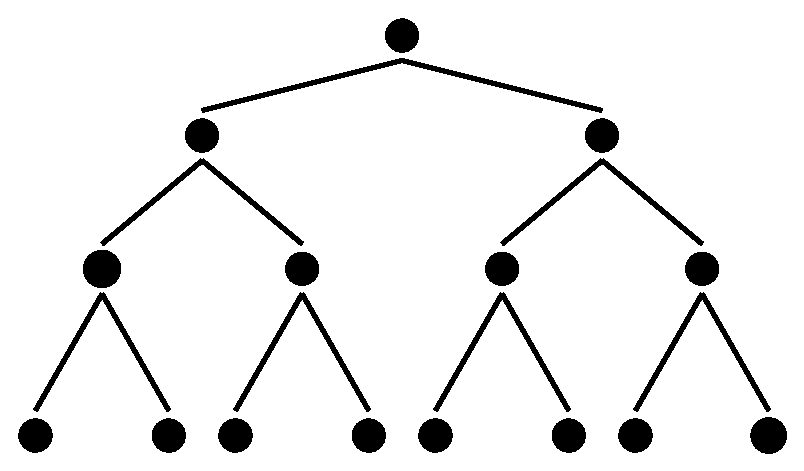
\includegraphics[width=0.4\textwidth]{fig/merging/huffman-1-trim}
	\caption{\label{tree:merging:fig/huffman-1} Initial state of the merge sort algorithm.}
\end{figure}

\begin{figure}
	\centering
	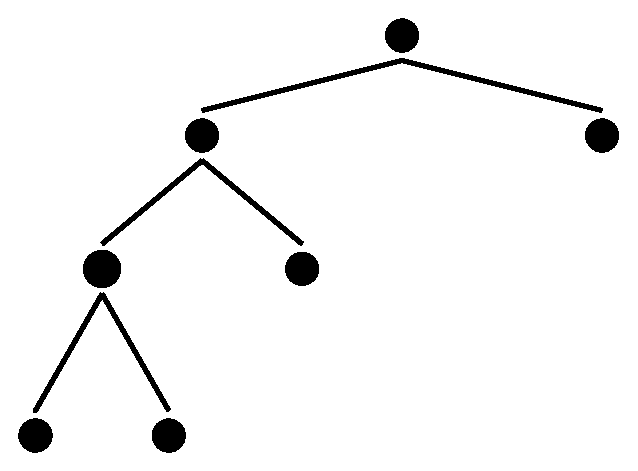
\includegraphics[width=0.4\textwidth]{fig/merging/huffman-3-trim}
	\caption{\label{tree:merging:fig/huffman-3} Intermediary state of the merge sort algorithm.}
\end{figure}

We can visualize the execution of merge sort as a tree that shrinks up to the root as the algorithm progresses to the solution. \ref{tree:merging:fig/huffman-1} shows the algorithm in the initial state $k = n, i = 1$. \ref{tree:merging:fig/huffman-3} shows the algorithm in an intermediary state where some totally ordered sets have been merged. Notice that this intermediary tree, where deeper leaves corresponds to smaller subsets, ressembles much like a Huffman tree (see \cite{huffman1952method}). From the beginning we assumed that $k = 2^m$ for some natural integer $m$. But this was wihout loss of generality since even for a non \emph{dyadic distribution} ($p(u) = 2^{-n_u}, n_u \in \mathbb{N}$, see \cite{cover2012elements}) the Huffman code is optimal.

The algorithm is thus building the huffman tree and then merge the two deepest leaves of the huffman tree until there is only one left.

\begin{figure}
	\centering
	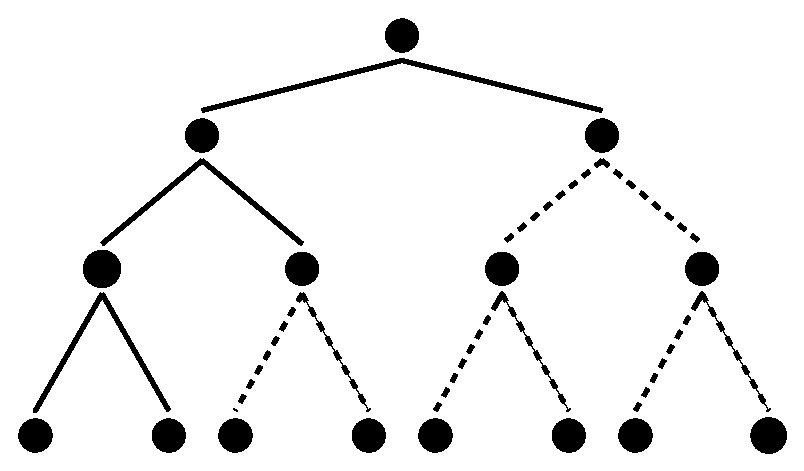
\includegraphics[width=0.4\textwidth]{fig/merging/huffman-2-trim}
	\caption{\label{tree:merging:fig/huffman-2} Complexity of the merging problem as a difference between the whole merge process and it's subprocesses.}
\end{figure}

Looking at \ref{tree:merging:fig/huffman-2} we can deduce the complexity of the algorithm. Since the dashed steps do not need to be processed and since the complexity of the merge sort is $\BigO{n \log n}$ we have a total complexity of $\BigO{n \log n - \sum_{i=1}^{k} n_i \log n_i} = \BigO{ITLB}$ where $n_i$ is the cardinality of the $i$-th totally ordered set of the input.




